\documentclass[10pt, dvipsnames]{beamer}
\usepackage[utf8x]{inputenc}
\usepackage{hyperref}
\usepackage{mtpro2}  % requires mtpro2 font
\usepackage{graphicx}
\usepackage[english,ngerman]{babel}
\usepackage{setspace}
\usepackage{enumitem}
\usepackage{xifthen, xargs}
\usepackage{mathtools, amsthm, amsfonts, siunitx, physics, chemformula, empheq}
\usepackage{animate}

\graphicspath{ {./Graphics/} }
% ------------------------------------------------------------------------------
% Use the beautiful metropolis beamer template
% ------------------------------------------------------------------------------
\usepackage[T1]{fontenc}
\usepackage{fontawesome5}
\usepackage{FiraSans} 
\mode<presentation>
{
	\usetheme[progressbar=foot,numbering=fraction,background=light]{metropolis} 
	\usecolortheme{default} % or try albatross, beaver, crane, ...
	\usefonttheme{serif}  % or try serif, structurebold, ...
	\setbeamertemplate{navigation symbols}{}
	\setbeamertemplate{caption}[numbered]
	\setbeamertemplate{section in toc}[sections numbered]
	%\setbeamertemplate{frame footer}{My custom footer}
} 
\setitemize{label=\usebeamerfont*{itemize item}%
	\usebeamercolor[fg]{itemize item}
	\usebeamertemplate{itemize item}}

% integral command
\ExplSyntaxOn
\NewDocumentCommand{\uint}{>{\SplitArgument{1}{,}}D[]{-,-} m m}{%
	\ifthenelse{\equal{\use_i:nn#1}{-}}
	{\int#2\, \dd#3}
	{\int\limits\c_math_subscript_token{\use_i:nn#1}\c_math_superscript_token{\use_ii:nn#1}#2 \,\dd#3}
}
\ExplSyntaxOff

% ------------------------------------------------------------------------------
% tcolorbox / tcblisting
% ------------------------------------------------------------------------------
\usepackage{xcolor}
\definecolor{codecolor}{HTML}{FFC300}

\usepackage{tcolorbox}
\tcbuselibrary{most}

\tcbset{tcbox width=auto,left=0mm,top=1mm,bottom=1mm,
	right=0mm,boxsep=1mm,middle=1pt}

\newtcolorbox{myr}{colback=codecolor!5,colframe=codecolor!80!black,
	left=1mm, right=1mm, enhanced, fonttitle=\bfseries}

\newtcolorbox{myr2}{colback=lime!5,colframe=lime!80!black,
	left=1mm, right=1mm, enhanced, fonttitle=\bfseries}

\newcommand*\s[1]{\textcolor{RoyalBlue}{#1}}
\newcommand*\zz[1]{\sum_{n = 1}^{\infty} \tfrac{1}{n^{\s{#1}}} = \tfrac{1}{1^{\s{#1}}} + \tfrac{1}{2^{\s{#1}}} + \tfrac{1}{3^{\s{#1}}} + \cdots}
\newcommand*{\iu}{{i\mkern1mu}}

\title{Riemann zeta function}
\author{Alexander Helbok, Matthias Lotze, Patryk Morawski, Helen Zwölfer}
\date{\today}

\begin{document}
	\setbeamertemplate{caption}{\raggedright\insertcaption\par}
	
	\maketitle
	\begin{frame}[noframenumbering, plain]{Overview}
		\tableofcontents
	\end{frame}

	\section{Introduction to the zeta function}	
	\begin{frame}[t]{Definition}
		\vspace{0.6cm}
		\begin{myr}
			\[ \zeta(\s{s}) = \zz{s} \qquad, \text{for }\operatorname{Re}(\s{s}) > 1\] 
		\end{myr} \vspace{2em}
		\begin{minipage}{\textwidth}
			\hspace{0.5cm}
			\only<2>{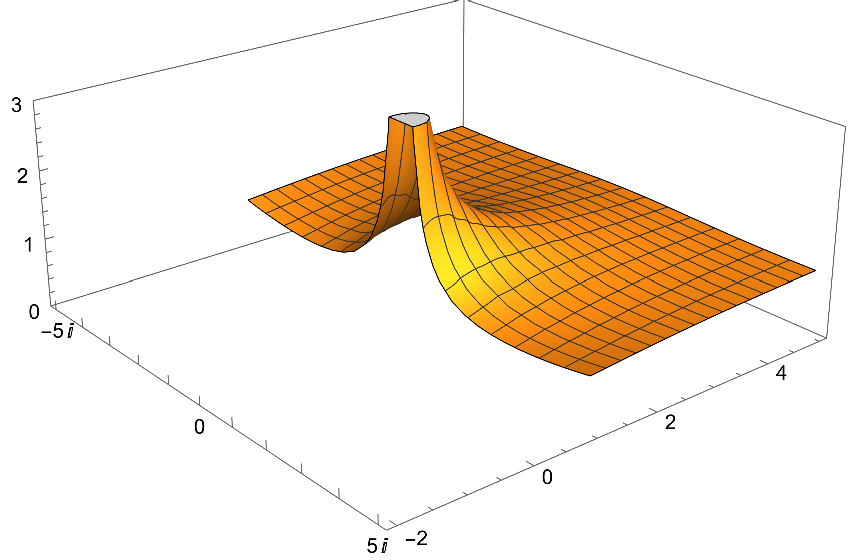
\includegraphics[scale=0.35]{PlotZeta}}
			\only<3-4>{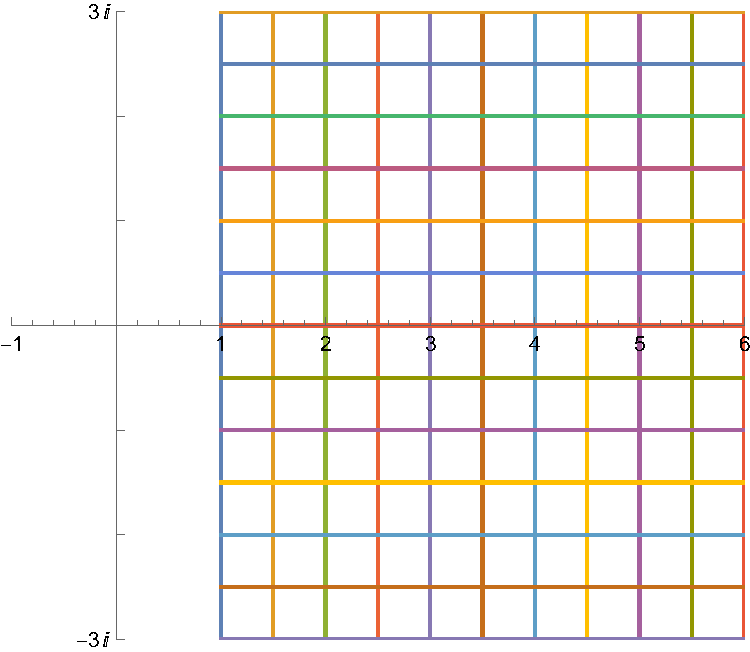
\includegraphics[scale=0.3]{Grid1}
			\hspace{0.3cm}
			\begin{minipage}{0.1\textwidth}
				\vspace{-3cm}\Huge\( \Rightarrow \)
			\end{minipage}}
			\hspace{0.3cm}
			\only<4>{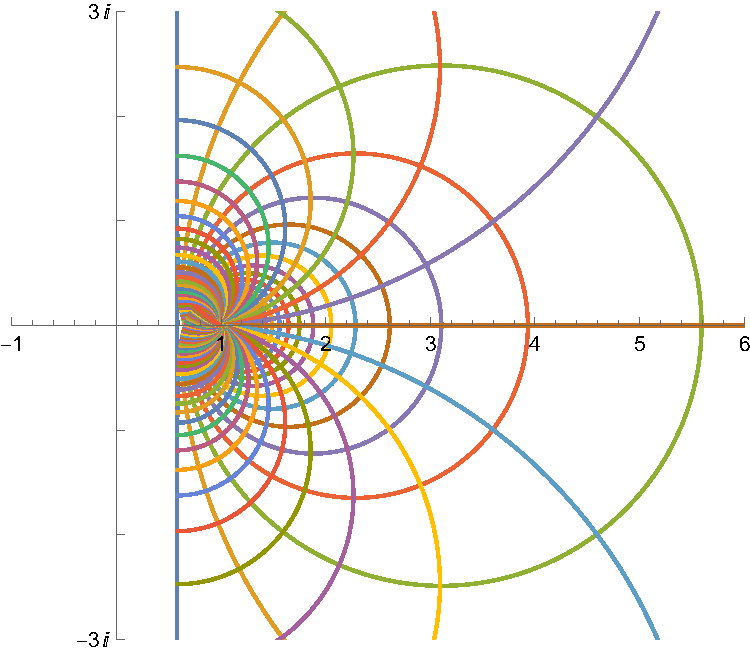
\includegraphics[scale=0.3]{Zeta1}}
			\only<5>{\hspace{0.5cm}\animategraphics[loop,controls,width=0.65\linewidth]{10}{/Anim/anim-}{0}{89}}
		\end{minipage}
	\end{frame}

	\begin{frame}[t]{Properties}
		\begin{itemize}[label={--}]
 			\uncover<1-6>{\item meromorphic (holomorphic with pole at s = 1)}
			\uncover<2-6>{\item complex differentiable in \( \mathbb{C} \Rightarrow \) analytic + infinitely differentiable}
			\uncover<3-6>{\item unique analytic continuation}
			\uncover<5-6>{\item conformal (preserves Angles)} 
			\uncover<6>{\item symmetric along real axis}
		\end{itemize}
		\begin{minipage}{\textwidth}
			\hspace{0.5cm}
			\only<1>{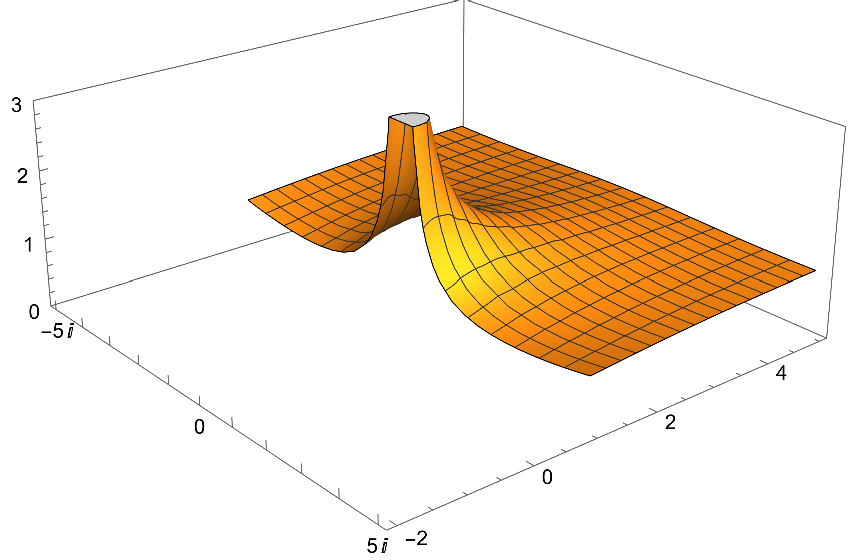
\includegraphics[scale=0.35]{PlotZeta}}
			\only<3>{\hspace{0.13cm}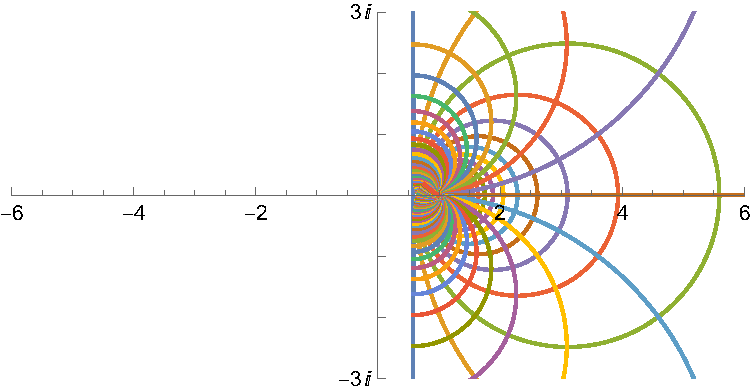
\includegraphics[scale=0.4]{extended1}}
			\only<4>{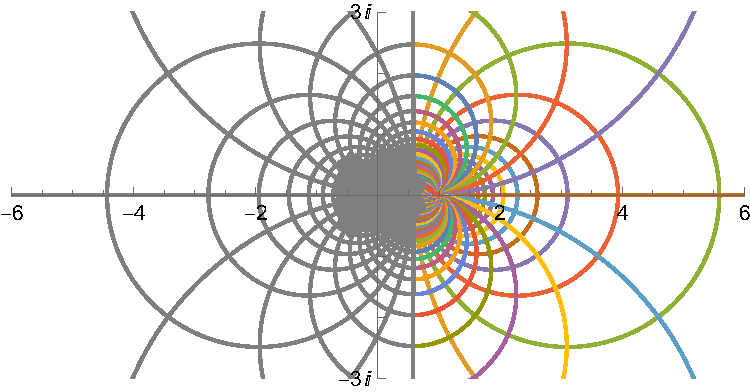
\includegraphics[scale=0.4]{extended2}}
			
			\hspace{0.5cm}
			\only<5>{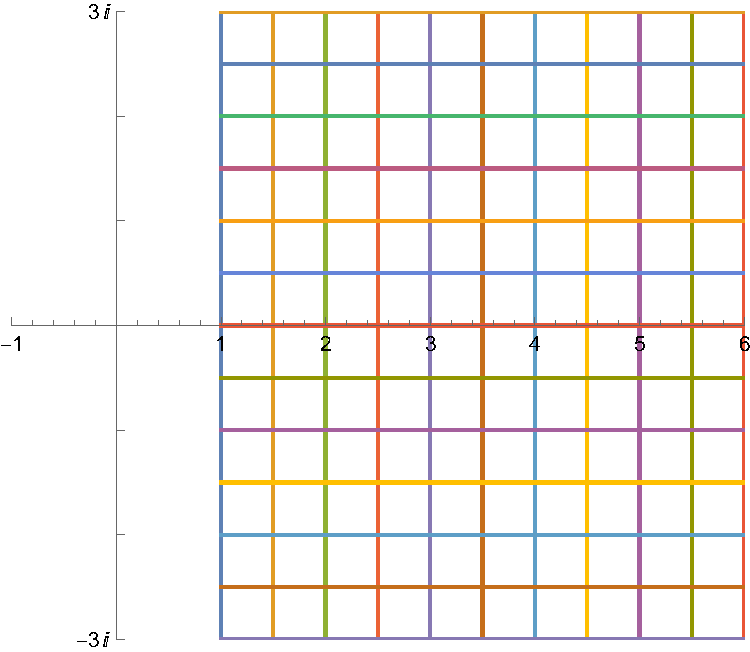
\includegraphics[scale=0.28]{Grid1}
			\hspace{0.3cm}
			\begin{minipage}{0.1\textwidth}
				\vspace{-3cm}\Huge\( \Rightarrow \)
			\end{minipage}}
			\hspace{0.3cm}
			\only<5>{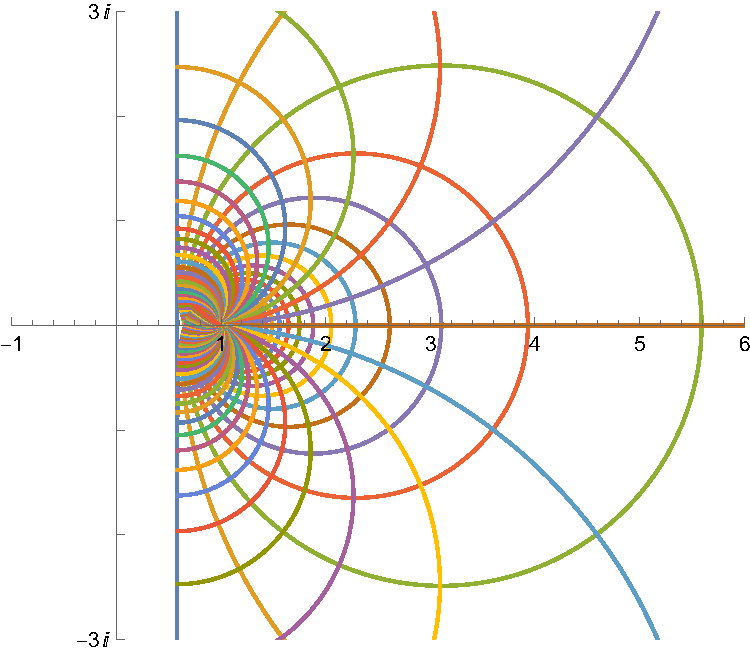
\includegraphics[scale=0.28]{Zeta1}}
			
			\only<6>{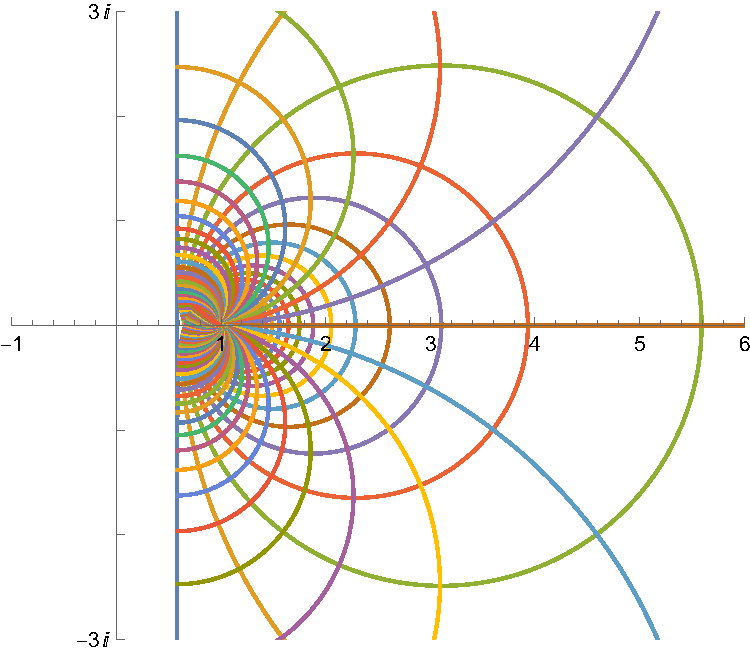
\includegraphics[scale=0.3]{Zeta1}
			\hspace{1cm}
			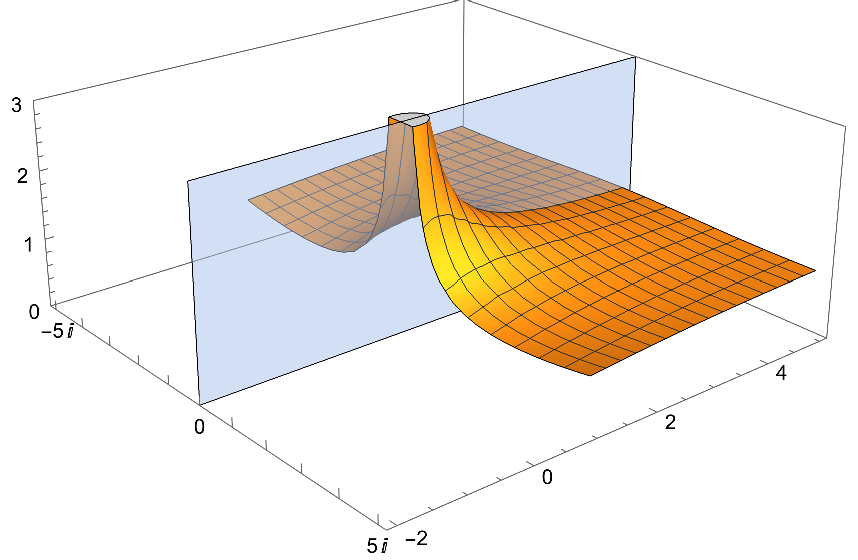
\includegraphics[scale=0.35]{PlotZeta2}}
		\end{minipage}
	\end{frame}

	\begin{frame}{A few values}
		\begin{myr}
			\begin{align*}
				&\zeta(\s{1}) = \uncover<2-14>{\zz{1} =} \uncover<3-14>{ \infty \hspace{1.2cm} (\text{harmonic Series}) }\\
				&\uncover<4-14>{\zeta(\s{2}) =} \uncover<5-14>{ \zz{2} =}\uncover<6-14>{ \frac{\pi^2}{6} \hspace{1.25cm} (\text{Basel Problem}) }\\
				&\uncover<7-14>{\zeta(\s{3 + \iu}) =} \uncover<8-14>{ \zz{3 + \iu}}\uncover<9-14>{ \approx 1.107 - 0.148 \iu} \\
				&\uncover<10-14>{\zeta(\s{-1}) =} \uncover<12-14>{ \sum_{n = 1}^{\infty} \tfrac{1}{n^{\s{-1}}} = 1 + 2 + 3 + 4 + \cdots =} \uncover<14>{\text{undefined!}}\\
			\end{align*}
		\end{myr}
		\hspace{1.608cm}
		\begin{minipage}{0.2\textwidth}
			\vspace{-4.4cm}
			\[ \only<11>{\zz{-1} =} \]
		\end{minipage}
		\hspace{2.65cm}
		\begin{minipage}{0.2\textwidth}
			\vspace{-4.58cm}
			\[ \only<13>{-\tfrac{1}{12} \hspace{2.2cm} (\text{???}) } \]
		\end{minipage}
	\end{frame}

	\section{Riemann conjecture}
	\begin{frame}{General Introduction to the Riemann Hypothesis}
		\vspace{0.3cm}
		\begin{myr}
			\[ \zeta(s) = \sum_{n = 1}^{\infty} \tfrac{1}{n^{s}} \qquad \text{for }s = \sigma+\iu t \ \text{ with } \sigma > 1 \] 
		\end{myr}
	    \begin{myr2}
	    	„All nontrivial zeros of the Riemann zeta function have real part \( \frac{1}{2} \)”
	    \end{myr2}
		\begin{itemize}[label={--}]
			\item Proposed by Riemann in 1859
			\item One of the Clay Mathematic Institute's Millennium Prize Problems, which offers a million dollars to anyone who solves any of them
		\end{itemize}
		To even consider the Riemann zeta function for \( s \in \mathbb{C} \) with \( \operatorname{Re}(s) = \sigma < 1 \), we first need to find a definition \\ \( \Rightarrow \) Analytic Continuation
	\end{frame}

	\begin{frame}{Alternative formula}
		\begin{myr}\centering
			\( \Gamma(s) = \uint[0, \infty]{x^{s-1} \exp[-x]}{x} \)
		\end{myr}
		The Gamma function is a generalization of the factorial: \\
		
		\( \Gamma(1) = 1 \) and \( n\Gamma(n) = \Gamma(n + 1) \)(integration by parts) \\
		\( \Rightarrow \Gamma(n + 1) = n! \text{ for } n \in \mathbb{N}\) \\[1em]
		
		Now we substitute \( n u=x \), thus \( n \dd u = \dd x \) in the Gamma function: \\
		\( \Gamma(s) = \uint[0, \infty]{x^{s-1} \exp[-x]}{x} \stackrel{\text{u-sub}}{=}
	    \uint[0, \infty]{n^{s} u^{s-1} \exp[-nu]}{u} \) 
	\end{frame}
	\begin{frame}{Analytic Continuation and Functional Equation of \( \zeta(s) \)}
		Taking the sum of \( \tfrac{\Gamma(s)}{n^{s}} \) we get: 
		\[ \sum_{n = 1}^{\infty} \tfrac{\Gamma(s)}{n^{s}} = \sum_{n = 1}^{\infty}\left[ \uint[0, \infty]{x^{s-1} \exp[-nx]}{x} \right] \stackrel{(*)}{=} \uint[0, \infty]{\left[\sum_{n = 1}^{\infty} \exp[-nx] \right] x^{s-1} }{x} \] 
		(\( * \)) We can change the order of summation and integration because of absolute convergence \\[2em]
		
		\( \sum_{n = 1}^{\infty} \exp[-nx] \) is a geometric series \( \sum_{n = 1}^{\infty} p^n = \tfrac{p}{1 - p} \) with \( p = \exp[-nx] \). Therefore: \\[1em]
		\( \uint[0, \infty]{\left[\sum_{n = 1}^{\infty} \exp[-nx] \right] x^{s-1} }{x} = \uint[0, \infty]{\tfrac{\exp[-x]}{1 - \exp[-x]} x^{s-1} }{x} = \uint[0, \infty]{\tfrac{x^{s-1}}{\exp[-x] - 1}}{x} \)\\
		Now we have: \( \Gamma(s)\zeta(s) = \uint[0, \infty]{\tfrac{x^{s-1}}{\exp[-x] - 1}}{x}\ \text{for } \operatorname{Re}(s) = \sigma < 1 \)
	\end{frame}
	\begin{frame}{Analytic Continuation}
		\begin{myr}\centering
			Let the function \( f_0:K_0 \to \mathbb{C} \) be holomorphic
		\end{myr}
		\begin{itemize}
			\item Choose a point \( a_1 \in U \) and develop the power series \\
			\( \Rightarrow \) new function \( f_1 \) with convergence disk \( K_1 \), holomorphic on \( K_1 \)
			\item Choose \( a_2 \in K1\setminus K_0 \) and get \( f_2 \) with convergence disk \( K_2 \), holomorphic on \( K_2 \)
			\item \dots
		\end{itemize}
        \centering 
	    \begin{minipage}{0.6\textwidth}
	    	\hspace{1cm}
	    	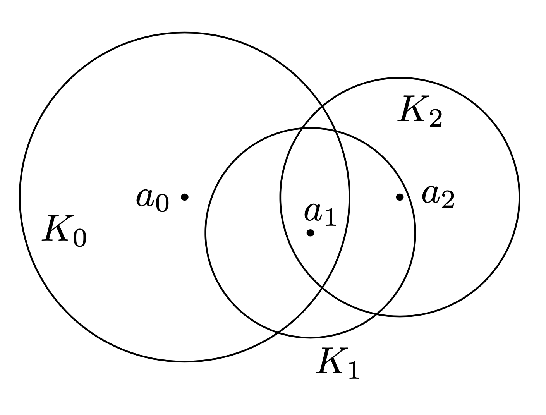
\includegraphics[scale=0.4]{cont}
	    \end{minipage}
        \\[0.2cm]
		Since \( f_i|_{K_i\cap K_j} = f_j|_{K_i\cap K_j} \) for all \( i, j \) we get a well-defined analytical continuation of \( f_0 \) on \( K_0, K_1, \dots \)
	\end{frame}

	\begin{frame}{Analytic Continuation}
		We now continue $\zeta(s)$ analytically using contour integrals. \\
		Let $C$ be a contour consisting of the real axis from $+\infty$ to $\rho$, the circle with $|x|=\rho$, $0<\rho<2\pi$, and the real axis from $\rho$ to $+\infty$. \\
		\begin{center}
		\vspace{0.1cm}
		\begin{minipage}{0.45\textwidth}
			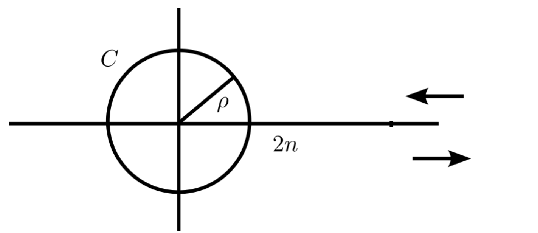
\includegraphics[scale=0.5]{int1}
		\end{minipage}\\[0.2cm]
		\end{center}
		We consider the Integral $I(s)=\int_C \frac{x^{s-1}}{\exp[x]-1} \dd{x}$. \\
		Reminder: We just proved $\Gamma(s)\zeta(s)=\sum_{n=1}^{\infty}\frac{\Gamma(s)}{n^s}=\int_{0}^{\infty}\frac{x^{s-1}}{\exp[x]-1} \dd{x}$ \\[1em]
		By the Residue Theorem, $I(s)$ cannot depend on $\rho$\\
		$\implies $ We can consider $\rho\rightarrow 0$ and deduce that the integral along the circle goes to zero. Thus only the paths along the real axis contribute. 
	\end{frame}
	
	\begin{frame}[t]{Analytic Continuation}
		Simplifying, we get $I(s)=\frac{\zeta(s)}{\Gamma(1-s)} 2\pi i\exp[\pi i s]$.\\
		$\implies \zeta(s)=\frac{\exp[-i\pi s]\Gamma(1-s)}{2\pi i} \int_C\frac{x^{s-1}}{\exp[x]-1} \dd{x}$ for $\sigma >1$ \\[1em]
		However, the integral converges uniformly for all s, so the only poles left are given by $\Gamma(1-s)$, thus for $s=1,2,3,...$. \\[1em]
		$I(s)$ vanishes for $s=2,3,...$ and therefore the only pole is at $s=1$. \\
		$\implies$ The function is holomorphic for $s\neq 1$. 
	\end{frame}
	
	\begin{frame}{Functional Equation}
		We now use the same technique of contour integrals to deduce a functional equation. Consider $I_n=\int_{C_n}\frac{x^{s-1}}{\exp[x]-1} \dd{x}$ along $C_n$. \\[0.2cm]
		\begin{center}
		\begin{minipage}{0.5\textwidth}
			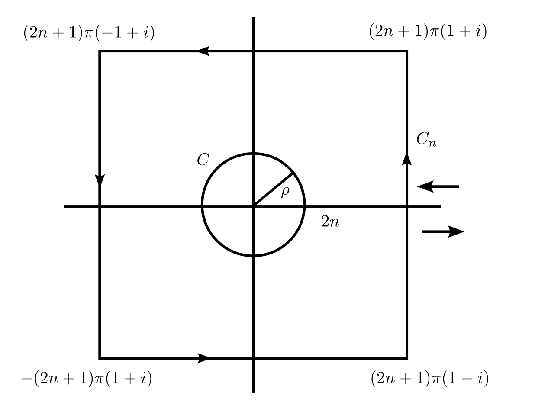
\includegraphics[scale=0.5]{int2}
		\end{minipage}\\[0.2cm]
		\end{center}
		Residue Theorem: $I(s)+2\pi i \sum \text{residues}=I_n(s)\iff I(s)=I_n(s)-2\pi i \sum \text{residues}$ \\
		Between $C$ and $C_n$ we have poles at $\pm 2i \pi$,...,$\pm 2n i \pi$. Calculating the residues, we get: $I(s)=I_n(s)+4\pi i \exp[i \pi s]\sin\left[\frac{\pi s}{2}\right]\sum_{m=1}^{n}(2m\pi)^{s-1}$
	\end{frame}

	\begin{frame}{Functional Equation}
		We now consider $\sigma <0$ and $n\rightarrow \infty$. Then $I_n(s)\rightarrow 0$. \\
%			\centering
%		\begin{minipage}{0.5\textwidth}
%			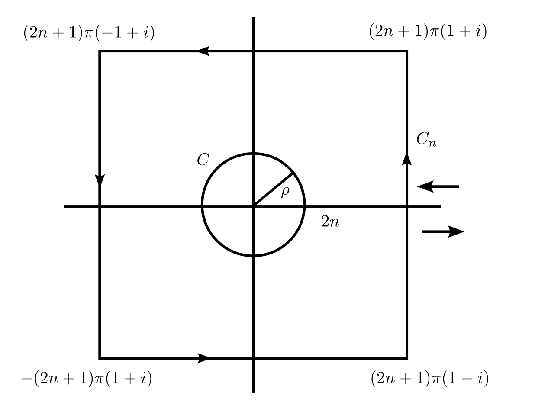
\includegraphics[scale=0.5]{int2}
%		\end{minipage}\\[0.2cm]
		We now have:\vspace{-0.25cm}
		\begin{equation*}
			\begin{split}
				I(s)
				&=4\pi i \exp[i \pi s]\sin\left[\frac{\pi s}{2}\right]\sum_{m=1}^{n}(2m\pi)^{s-1}\\
				&=4\pi i \exp[i \pi s]\sin\left[\frac{\pi s}{2}\right](2\pi)^{s-1}\zeta(1-s)
			\end{split}
		\end{equation*}
		\vspace{-0.1cm}
		\noindent Using $I(s)=\frac{\zeta(s)}{\Gamma(1-s)} 2\pi i\exp[\pi i s]$ which we got by analytic \\
		\hspace{0.05cm} continuation: 
		\begin{equation*}
			\begin{split}
				&  \frac{\zeta(s)}{\Gamma(1-s)} 2\pi i\exp[\pi i s]=I(s)=4\pi i \exp[i \pi s]\sin\left[\frac{\pi s}{2}\right](2\pi)^{s-1}\zeta(1-s)\\
				&\implies \zeta(s)=\Gamma(1-s)\zeta(1-s)2^s\pi^{s-1}\sin\left[\frac{\pi s}{2}\right]
			\end{split}
		\end{equation*}
		\vspace{-0.1cm}
		This functional equation holds for $\sigma <0$.\\
		\hspace{0.05cm}
		So we found the “trivial“ zeros at $s=-2m$, $m\in\mathbb{N}$!
	\end{frame}
	\begin{frame}{What have we accomplished?}
		\begin{itemize}[itemsep=10pt]
			\uncover<1-4>{\item $\zeta(s)=\sum_{n=1}^{\infty}\frac{1}{n^s}$ for $\sigma >1$. \\}
			\uncover<2-4>{\item $\Gamma(s)\zeta(s)=\int_0^\infty \frac{x^{s-1}}{\exp[x]-1} \dd{x}$ for $\sigma >1$ \\}
			\uncover<3-4>{\item Analytic continuation via contour integral: \\
			$\zeta(s)=\frac{\exp[-i\pi s]\Gamma(1-s)}{2\pi i}\int_C\frac{x^{s-1}}{\exp[x]-1} \dd{x}$ \\} 
			\uncover<4>{\item Functional equation by considering residues: \\
			$\zeta(s)=\Gamma(1-s)\zeta(1-s)2^s\pi^{s-1}\sin\left[\frac{\pi s}{2}\right]$ for $\sigma <0$}
			\uncover<3-4>{
			\begin{minipage}{0.45\textwidth}
				\vspace{0.3cm}
				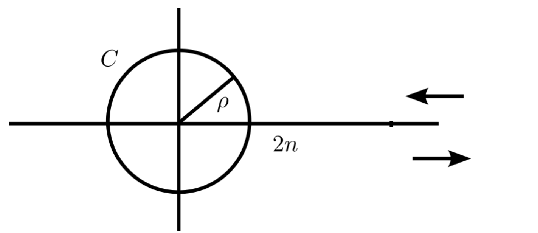
\includegraphics[scale=0.5]{int1}
			\end{minipage}}	
			\uncover<4>{
			\begin{minipage}{0.45\textwidth}
				\vspace{0.3cm}
				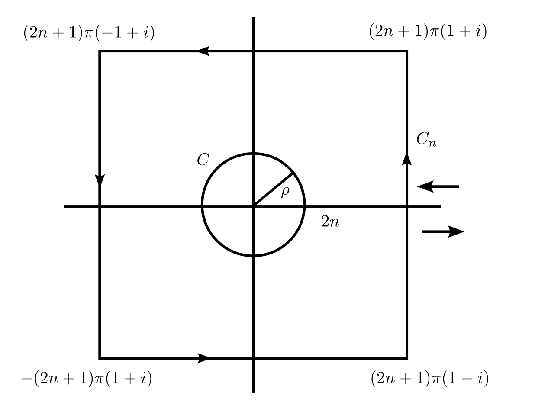
\includegraphics[scale=0.43]{int2}
			\end{minipage}}	
		\end{itemize}
	\end{frame}

	\section{Zeta function and primes}
	\begin{frame}{Prime step-function}
		\animategraphics[loop,controls=play,width=\linewidth]{10}{/anim2/anim-}{0}{200}
	\end{frame}
	
	\section{Formal definitions}
	\begin{frame}{(Algebraic) field $(K, +, \cdot)$}
		\begin{itemize}[label={--}, itemsep=10pt]
			\item $+, \cdot: K \times K \to K$ 
			\item $(K, +)$ abelian group 
			\item $(K \setminus \{ 0\}, \cdot)$ abelian group 
		\end{itemize} 
	\end{frame}

	\begin{frame}{$K$-Vector space $(V, \oplus, \odot)$}
		\begin{itemize}[label={--}, itemsep=10pt]
			\item $\oplus: V \times V \to V \quad \Rightarrow $  $(V, \oplus)$ abelian group 
			\item $\odot : K \times V \to V \quad \Rightarrow$ scalar multiplication of the field $K$ on $(V, \oplus)$ 
			\item $\text{Hom} (V, W) := \{f \mid f: V \to W \} $: 
			\begin{align*}
				(f, g) &\mapsto f \oplus g \\
				V \ni v &\mapsto (f \oplus g) (v) := f(v) + g(v) \in W \\ 
				(\lambda, f) &\mapsto \lambda \odot f \\ 
				V \ni v &\mapsto (\lambda \odot f) (v):= \lambda f(v) \in W 
			\end{align*}
		\end{itemize} 
	\end{frame}

	\begin{frame}{Algebra $(A, +, \cdot, \bullet)$}
		\begin{itemize}[label={--}, itemsep=10pt] 
			\item $(A, +, \cdot)$ $K$-Vector space 
			\item $\bullet: A \times A \to A$ product on $A \Rightarrow$ $K$-bilinear map 
			\item $(C^\infty(M), +, \cdot, \bullet)$: associative, unital, commutative algebra over $\mathbb{R}/ \mathbb{C}$ 
			\begin{align*}
				\bullet: C^\infty (M) \times C^\infty (M) &\to C^\infty (M) \\
				(f, g) &\mapsto f \bullet g \\ 
				M \ni v &\mapsto (f\bullet g) (v) := f(v) \cdot g(v) 
			\end{align*}
		\end{itemize} 
	\end{frame}

	\maketitle
\end{document} 
